\documentclass[
	a4paper,
	oneside,
	BCOR = 10mm,
	DIV = 12,
	12pt,
	headings = normal,
]{scrartcl}

%%% Length calculations
\usepackage{calc}
%%%

%%% Support for color
\usepackage{xcolor}
\definecolor{lightblue}{HTML}{03A9F4}
\definecolor{red}{HTML}{F44336}
%%%

%%% Including graphics
\usepackage{graphicx}
%%%

%%% Font selection
\usepackage{fontspec}

\setromanfont{STIX Two Text}[
	SmallCapsFeatures = {LetterSpace = 8},
]

\setsansfont{IBM Plex Sans}[
	Scale = MatchUppercase,
]

\setmonofont{IBM Plex Mono}[
	Scale = MatchUppercase,
]
%%%

%%% Math typesetting
\usepackage{amsmath}

\usepackage{unicode-math}
\setmathfont{STIX Two Math}

\usepackage{IEEEtrantools}
%%%

%%% List settings
\usepackage{enumitem}
\setlist[enumerate]{
	label*      = {\arabic*.},
	leftmargin  = *,
	labelindent = \parindent,
	topsep      = 1\baselineskip,
	parsep      = 0\baselineskip,
	itemsep     = 1\baselineskip,
	noitemsep, % override itemsep
}

\setlist[itemize]{
	label*      = {—},
	leftmargin  = *,
	labelindent = \parindent,
	topsep      = 1\baselineskip,
	parsep      = 0\baselineskip,
	itemsep     = 1\baselineskip,
	noitemsep, % override itemsep
}

\setlist[description]{
	font        = {\rmfamily\upshape\bfseries},
	topsep      = 1\baselineskip,
	parsep      = 0\baselineskip,
	itemsep     = 0\baselineskip,
}

\newlist{steps}{enumerate}{10}
\setlist[steps]{
	label*      = {\arabic*.},
	leftmargin  = 0em,
	labelindent = \parindent,
	topsep      = 1\baselineskip,
	parsep      = 0\baselineskip,
	itemsep     = 1\baselineskip,
	noitemsep, % override itemsep
}


%%%

%%% Structural elements typesetting
\setkomafont{pagenumber}{\rmfamily\upshape}
\setkomafont{disposition}{\rmfamily\bfseries}

% Sectioning
\RedeclareSectionCommand[
	beforeskip = -1\baselineskip,
	afterskip  = 1\baselineskip,
	font       = {\normalsize\bfseries\scshape},
]{section}

\RedeclareSectionCommand[
	beforeskip = -1\baselineskip,
	afterskip  = 1\baselineskip,
	font       = {\normalsize\bfseries\itshape},
]{subsection}

\RedeclareSectionCommand[
	beforeskip = -1\baselineskip,
	afterskip  = 1\baselineskip,
	font       = {\normalsize\bfseries},
]{subsubsection}

\RedeclareSectionCommand[
	beforeskip = -1\baselineskip,
	afterskip  = -0.5em,
	font       = {\normalsize\mdseries\scshape\addfontfeatures{Letters = {UppercaseSmallCaps}}},
]{paragraph}
%%%

%%% Typographic enhancements
\usepackage{microtype}
%%%

%%% Language-specific settings
\usepackage{polyglossia}
\setmainlanguage{ukrainian}
\setotherlanguages{english}
%%%

%%% Captions
\usepackage{caption}
\usepackage{subcaption}

%\DeclareCaptionLabelFormat{closing}{#2)}
%\captionsetup[subtable]{labelformat = closing}

%\captionsetup[subfigure]{labelformat = closing}

\captionsetup[table]{
	aboveskip = 0\baselineskip,
	belowskip = 0\baselineskip,
}

\captionsetup[figure]{
	aboveskip = 1\baselineskip,
	belowskip = 0\baselineskip,
}

\captionsetup[subfigure]{
	labelformat = simple,
	labelformat = brace,
}
%%%

%%% Hyphenated ragged typesetting
\usepackage{ragged2e}
%%%

%%% Table typesetting
\usepackage{booktabs}
\usepackage{longtable}

\usepackage{multirow}

\usepackage{array}
\newcolumntype{v}[1]{>{\RaggedRight\arraybackslash\hspace{0pt}}p{#1}}
\newcolumntype{b}[1]{>{\Centering\arraybackslash\hspace{0pt}}p{#1}}
\newcolumntype{n}[1]{>{\RaggedLeft\arraybackslash\hspace{0pt}}p{#1}}
%%%

%%% Drawing
\usepackage{tikz}
\usepackage{tikzscale}
\usetikzlibrary{positioning}
\usetikzlibrary{arrows.meta} % Stealth arrow tips
%%%

%%% SI units typesetting
\usepackage{siunitx}
\sisetup{
	output-decimal-marker = {,},
	exponent-product      = {\cdot},
	inter-unit-product    = \ensuremath{{} \cdot {}},
	per-mode              = symbol,
}
%%%

%%% Framing code listings
\usepackage{tcolorbox}
\tcbuselibrary{breakable}
\tcbuselibrary{minted}
\tcbuselibrary{skins}

\newtcblisting[
	auto counter, 
	list inside, 
	number within = section,
]{listingprolog}[3][]{%
	minted language = prolog,
	minted style    = bw,
	minted options  = {
		linenos,
		tabsize = 4,
		breaklines,
		% breakanywhere,
		fontsize = \footnotesize,
		autogobble
	},
	%
	empty,
	sharp corners,
	coltitle              = black,
	borderline horizontal = {1pt}{0pt}{black},
	titlerule             = 0.5pt,
	titlerule style       = {
		black,
	},
	toptitle         = 0.3em,
	bottomtitle      = 0.1em,
	before skip      = \intextsep,
	after  skip      = \intextsep,
	title            = {Лістинг \thetcbcounter: #2},
	list entry       = {\protect\numberline{\thetcbcounter}#2},
	left = 0em,
	right = 0em,
	%
	listing only,
	breakable,
	%
	label = {#3},
	%
	#1
}

\newtcbinputlisting[auto counter, list inside, number within = section]{\inputprolog}[4][]{%
	minted language = prolog,
	minted style    = bw,
	minted options  = {
		linenos,
		tabsize = 4,
		breaklines,
		breakbytokenanywhere,
		fontsize = \footnotesize,
	},
	%
	empty,
	sharp corners,
	coltitle              = black,
	borderline horizontal = {1pt}{0pt}{black},
	titlerule             = 0.5pt,
	titlerule style       = {
		black,
	},
	toptitle         = 0.3em,
	bottomtitle      = 0.1em,
	before skip      = \intextsep,
	after  skip      = \intextsep,
	title            = {Лістинг \thetcbcounter: #3},
	list entry       = {\protect\numberline{\thetcbcounter}#3},
	left = 0em,
	right = 0em,
	%
	listing file={#2},
	listing only,
	breakable,
	%
	label = {#4},
	%
	#1
}

% Customize minted
\usepackage{minted}
\setminted{
	style = bw,
	breaklines,
	linenos,
}

\setmintedinline{
	style = bw,
	breaklines,
}

% Customize minted line numbers
\renewcommand{\theFancyVerbLine}{\ttfamily\scriptsize\arabic{FancyVerbLine}}

%%%

%%% Keystroke typesetting
\usepackage[
	os = win,
]
{menukeys}
%%%

%%% Links and hyperreferences
\usepackage{hyperref}
\hypersetup{
	bookmarksnumbered = true,
	colorlinks      = false,
	linkbordercolor = red,
	urlbordercolor  = lightblue,
	pdfborderstyle  = {/S/U/W 1.5},
}
%%%

%%% Length adjustments
% Set baselineskip, default is 14.5 pt
\linespread{1.068966} % ~15.5 pt
\setlength{\emergencystretch}{1em}
\setlength{\parindent}{1.5em}
\newlength{\gridunitwidth}
\setlength{\gridunitwidth}{\textwidth / 12}
%%%

%%% Custom commands
\newcommand{\allcaps}[1]{{\addfontfeatures{LetterSpace = 8, Kerning = Off}#1}}
\newcommand{\filename}[1]{\texttt{#1}}
\newcommand{\progname}[1]{\texttt{#1}}
\newcommand{\modulename}[1]{\texttt{#1}}

\newcommand{\userinput}[1]{\texttt{#1}}

\newcommand{\Mytextrightarrow}{$\rightarrow$}
%%%

%%% Custom math commands
\newcommand{\longvar}[1]{\mathit{#1}}
%%%

\begin{document}

\begin{titlepage}
		\begin{center}
			Міністерство освіти і науки України\\
			Національний авіаційний університет\\
			Навчально-науковий інститут комп'ютерних інформаційних технологій\\
			Кафедра комп'ютеризованих систем управління

			\vspace{\fill}
				Лабораторна робота~№1\\
				з~дисципліни «Функціональне і~логічне програмування»\\
				на~тему «Знайомство із~середовищем розробки~\textenglish{Turbo Prolog}»\\

			\vspace{\fill}

			\begin{flushright}
				Виконав:\\
				студент \allcaps{ННІКІТ}\\
				групи СП-325\\
				Клокун В.\,Д.\\
				Перевірила:\\
				Клобукова С.\,М.
			\end{flushright}

			Київ 2019
		\end{center}
	\end{titlepage}

	\section{Мета роботи}
		Оволодіти основами роботи в~середовищі~\textenglish{Turbo Prolog}.
	
	\section{Завдання роботи}
		Запустити середовище~\textenglish{Turbo Prolog}; ознайомитись з~призначенням вікон, пунктами меню та~основними прийомами керування середовищем. 

	\section{Хід роботи}
		Встановлюємо середовище розробки~\textenglish{Turbo Prolog}.  Щоб~встановити середовище, розпаковуємо вміст архіву з~\textenglish{Turbo Prolog} у~відповідну папку. Тепер середовище~\textenglish{Turbo Prolog} встановлене.
		
		Запускаємо встановлене середовище. Щоб запустити середовище, запускаємо програму~\textenglish{\allcaps{DOSBOX}} і~монтуємо папку, яка містить середовище~\textenglish{Turbo Prolog}, як~диск~«\textenglish{C:}». Для цього у~вікні~\textenglish{\allcaps{DOSBOX}} вводимо таку команду:
		\begin{minted}{batch}
mount c <шлях до TurboProlog>
		\end{minted}
		Змонтувавши необхідну папку як~диск, переходимо в~нього і~запускаємо середовище. Для~цього у~вікні~\textenglish{\allcaps{DOSBOX}} виконуємо таку команду:
		\begin{minted}{batch}
C:
PROLOG.exe
		\end{minted}
		В~результаті у~вікні~\textenglish{\allcaps{DOSBOX}} запуститься середовище програмування~\textenglish{Turbo Prolog}~(рис.~\ref{fig:turbo-prolog}). 
		
		\begin{figure}[!htbp]
			\begin{subfigure}[b]{0.5\columnwidth}
				\centering
				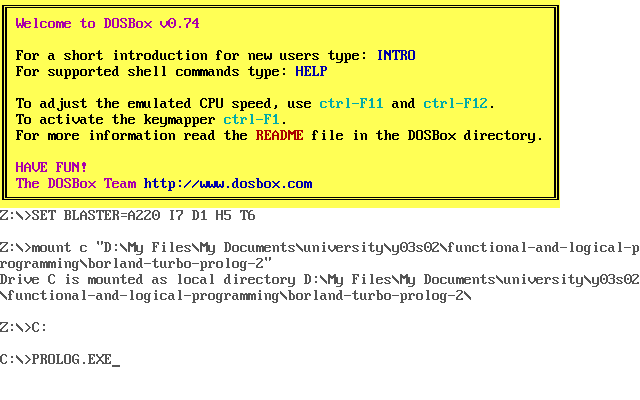
\includegraphics[width = \columnwidth]{./assets/y03s02-flp-lab-01-p01-neg.png}
				\caption{}
				\label{subfig:turbo-prolog-01}
			\end{subfigure}%
			~
			\begin{subfigure}[b]{0.5\columnwidth}
				\centering
				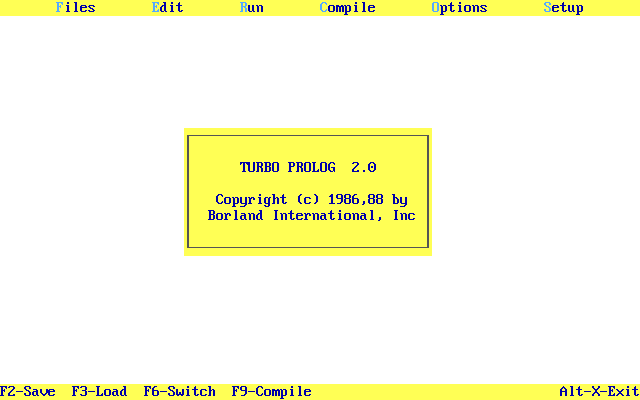
\includegraphics[width = \columnwidth]{./assets/y03s02-flp-lab-01-p02-neg.png}
				\caption{}
				\label{subfig:turbo-prolog-02}
			\end{subfigure}%
			\caption{Запуск середовища програмування~\textenglish{Turbo Prolog}}
			\label{fig:turbo-prolog}
		\end{figure}

		Розглядаємо вікно середовища~(рис.~\ref{fig:tprolog-win}) та~вивчаємо пункти його меню, основні прийоми роботи з~ним, оволодіваємо операціями автоматизованого пошуку і~заміни у~вікні редактора~\textenglish{Turbo Prolog}, прийомами копіювання тексту з~вікон~\textenglish{Turbo Prolog} до~програм~\textenglish{Microsoft Windows} і~навпаки.
		
		\begin{figure}[!htbp]
			\centering
			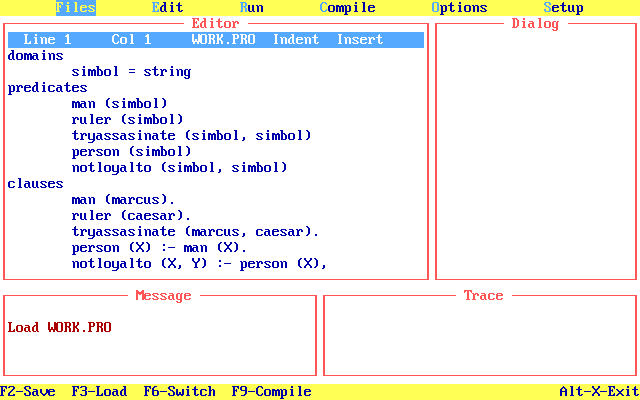
\includegraphics[height = 9\baselineskip]{./assets/y03s02-flp-lab-01-p03-neg.png}
			\caption{Вікно середовища~\textenglish{Turbo Prolog}}
			\label{fig:tprolog-win}
		\end{figure}

		Створюємо у~середовищі~\textenglish{Turbo Prolog} програму, яка~виведе повідомлення «\textenglish{Hello, World!}»~(лістинг~\ref{lst:hello-world}).

		\begin{listingprolog}{Програма для~виводу повідомлення~\textenglish{Hello, World!}}{lst:hello-world}
goal
	write("Hello, world!"),
	nl,
	exit.
		\end{listingprolog}

		Будуємо створену програму за~допомогою клавіші~\keys{F9}, а~потім запускаємо на~виконання, натиснувши комбінацію клавіш~\keys{\Alt + X}.

		\begin{figure}[!htbp]
			\centering
			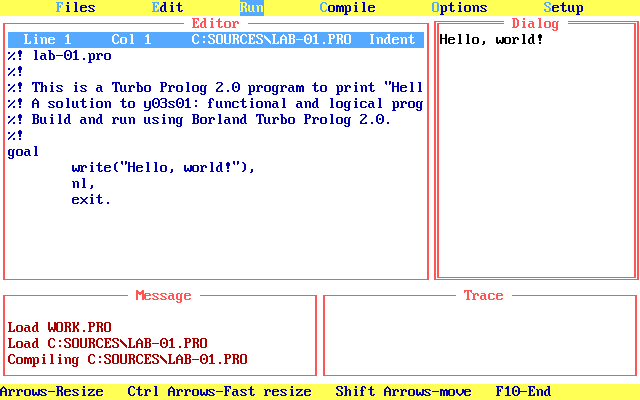
\includegraphics[height = 9\baselineskip]{./assets/y03s02-flp-lab-01-p04-neg.png}
			\caption{Результат виконання програми}
			\label{fig:hello-world-res}
		\end{figure}

		Спостерігаємо результат виконання програми у~вікні~\textenglish{Dialog}. Як~бачимо, розроблена програма успішно вивела рядок~«\textenglish{Hello, World!}».

	\section{Контрольні питання}
		\subsection{Скільки вікон має середовище~\textenglish{Turbo Prolog}? Назвіть їх.}
			Середовище~\textenglish{Turbo Prolog} має 4~вікна: 
			\begin{enumerate}
				\item \textenglish{Editor}~— вікно основного редактору, призначене для редагування початкового коду програм, які створюються у середовищі. 
				\item \textenglish{Dialog}~— вікно інтерпретатора, яке показує його вивід та діалогові запити на введення. 
				\item \textenglish{Message}~— вікно повідомлень, які~надсилає середовище розробки, серед яких можуть бути повідомлення про~завантаження файлів, компіляцію початкових кодів і~запуск скомпільованих програм. 
				\item \textenglish{Trace}~— вікно налагоджувача. 
			\end{enumerate}

		\subsection{Як в~середовищі~\textenglish{Turbo Prolog} перейти від одного вікна до іншого?}
			Щоб у~середовищі~\textenglish{Turbo Prolog} перейти від~одного вікна до~іншого, треба натиснути клавішу~\keys{F6}.

		\subsection{Що відображає нижній рядок вікна середовища~\textenglish{Turbo Prolog}?}
			У~середовищі~\textenglish{Turbo Prolog} нижній рядок вікна відображає підказки з~гарячими клавішами для~обраного елементу.

		\subsection{Як змінити розмір вікна в~середовищі~\textenglish{Turbo Prolog}?}
			Щоб~змінити розмір вікна у~середовищі~\textenglish{Turbo Prolog}, треба виділити бажане вікно, натискаючи клавішу~\keys{F6}, і, обравши бажане вікно, змінити його розмір, натискаючи клавіші~\keys{←}, \keys{↑}, \keys{→}, \keys{↓}.

		\subsection{Як розкрити активне вікно на весь екран?}
			Щоб розкрити активне вікно на весь екран, треба натиснути клавішу~\keys{F5}.

		\subsection{Як зберегти текст, написаний Вами у вікні редактора~\textenglish{Turbo Prolog}, в~файл під бажаною назвою?}
			Щоб зберегти текст, написаний у~вікні редактора~\textenglish{Turbo Prolog}, у~файл під~бажаною назвою, необхідно обрати пункт меню~«\textenglish{Files}»~\Mytextrightarrow{ } «\textenglish{Write to}».

		\subsection{Куди зберігається текст Вашої програми, якщо~натиснути~«\textenglish{File}»~— «\textenglish{Save}»?}
			Якщо натиснути~«\textenglish{File}»~\Mytextrightarrow{ } «\textenglish{Save}», текст у~вікні редактора зберігається у~файл, який зараз відкритий у~редакторі. 

		\subsection{Як відкрити у~вікні~\textenglish{Turbo Prolog} файл~\filename{C:\textbackslash{}Temp\textbackslash{}myfile.txt}?}
			Щоб відкрити у~вікні~\textenglish{Turbo Prolog} файл~\filename{C:\textbackslash{}Temp\textbackslash{}myfile.txt}, треба перейти в~пункт меню~«\textenglish{Files}»~\Mytextrightarrow{ } «\textenglish{Load}» і~ввести~\filename{C:\textbackslash{}Temp\textbackslash{}myfile.txt}.

		\subsection{Як відмітити початок і~кінець блоку?}
			Щоб відмітити початок блоку, необхідно перемістити курсор у~позицію бажаного початку блоку і~натиснути клавіші~\keys{\ctrl + Q}, \keys{K}. Щоб відмітити кінець блоку, необхідно перемістити курсор у~позицію бажаного кінця блоку і~натиснути клавіші~\keys{\ctrl + Q}, \keys{K}.

		\subsection{Як~скопіювати відмічений блок?}
			Щоб скопіювати відмічений блок, треба натиснути клавіші~\keys{\ctrl + K}, \keys{C}. 

		\subsection{Як~виконати пошук і~заміну елементів тексту?}
			Щоб почати пошук і~заміну елементів тексту, треба натиснути клавішу~\keys{F4} або~\keys{\ctrl + Q}, \keys{A}. Після натискання однієї з~комбінацій клавіш ~'явиться прохання ввести шуканий текст, який треба замінити. Туди необхідно ввести бажаний текст і~натиснути клавішу для~підтвердження. Якщо пошук і~заміна були початі клавішею~\keys{F4}, клавіша для~підтвердження~— \keys{F4}. Якщо~ж пошук і~заміна були початі клавішами~\keys{\ctrl + Q}, \keys{A}, клавіша для~підтвердження~— \keys{\return}. Після натискання клавіші підтвердження текст для~пошуку буде підтверджений, і~з'я\-ви\-ться прохання ввести текст, на~який шуканий текст буде замінений. Його необхідно ввести і~підтвердити так само, як~і~шуканий. 

			Після підтвердження тексту, на~який шуканий текст буде замінений, з'я\-ви\-ться вибір способу заміни: локальний або~глобальний. Щоб~обрати локальний пошук, необхідно натиснути клавішу~\keys{G}, щоб~обрати локальний~— клавішу~\keys{L}. Щоб~підтвердити вибір, треба натиснути~\keys{\return}.

			Після підтвердження способу заміни з'я\-ви\-ться вибір, чи~буде середовище запитувати дозвіл на~кожну заміну. Якщо треба запитувати дозвіл, треба натиснути клавішу~\keys{Y}, якщо ні~— клавішу~\keys{N}. Щоб перервати пошук і~заміну у~будь-який момент, треба натиснути~\keys{\esc}.

		\subsection{Чим відрізняється глобальний пошук від~локального?}
			Локальний пошук~(і~заміна, оскільки простий пошук завжди локальний) виконується до~першого знайденого шуканого слова, глобальний пошук і~заміна виконуються від~поточного положення курсору до~кінця відкритого файлу. 

		\subsection{Як користуватись вікном~«\textenglish{Aux Edit}»?}
			«\textenglish{Aux Edit}»~— це~вікно додаткового редактора, і~функціонально воно повністю ідентичне основному редактору. Щоб відкрити вікно додаткового редактора, треба спочатку перейти у~вікно основного редактора і~натиснути клавішу~\keys{F8}. В~результаті з'я\-ви\-ться вікно додаткового редактора, в~якому буде запропоновано обрати і~завантажити файл. Після завантаження файлу його можна редагувати, використовуючи ті~ж самі функції, що~і~у~вікні основного редактора. 

			Щоб закрити вікно додаткового редактору, треба натиснути клавішу~\keys{\esc}. Щоб~зберегти файл і~закрити вікно додаткового редактора, треба натиснути клавішу~\keys{F10}, вести бажане ім'я файлу та~натиснути~\keys{\return}.

		\subsection{Розгляньте відомі вам можливості копіювання тексту між~вікном~\textenglish{Turbo Prolog} та~текстовими редакторами, що~працюють під~\textenglish{Windows}~(\textenglish{Word}, Блокнот тощо)}
			Щоб~скопіювати текст з~вікна~\textenglish{Turbo Prolog}, запущеного безпосередньо під~управлінням~\textenglish{Microsoft Windows}, в~інші програми, можна скористатись меню командного рядка~«Змінити»~\Mytextrightarrow{ } «Копіювати». Для~цього треба:
			\begin{steps}
				\item Переключити програму у~віконний режим. 
				\item Натиснути лівою клавішею миші на~значок програми, який~знаходиться у~лівому верхньому кутку вікна. Після натиснення з'я\-ви\-ться випадаюче меню.
				\item У з'явившомуся меню вибрати пункти~«Змінити»~\Mytextrightarrow{ } «Виділити все». Тепер увесь вміст вікна буде виділений. 
				\item Натиснути лівою клавішею миші на~значок програми, який~знаходиться у~лівому верхньому кутку вікна. Після натиснення з'я\-ви\-ться випадаюче меню.
				\item У з'явившомуся меню вибрати пункти~«Змінити»~\Mytextrightarrow{ } «Копіювати». Тепер увесь вміст вікна буде скопійований у~буфер обміну. 
			\end{steps}
			Тепер бажаний текст знаходиться в~буфері обміну і~його можна вставляти у~будь-яку бажану програму. 

			Щоб~скопіювати текст з~інших програм у~вікно~\textenglish{Turbo Prolog}, запущеного безпосередньо під~управлінням~\textenglish{Microsoft Windows}, можна скористатись меню командного рядка~«Змінити»~\Mytextrightarrow{ } «Вставити». Для~цього треба:
			\begin{steps}
				\item У~потрібній програмі скопіювати текст у~буфер обміну будь-яким зручним способом. 
				\item Переключити програму~\textenglish{Turbo Prolog} у~віконний режим. 
				\item У~програмі~\textenglish{Turbo Prolog} перейти у~вікно~\textenglish{Edit}.
				\item Пересунути курсор на~ту~позицію, куди треба вставити скопійований текст. 
				\item Натиснути лівою клавішею миші на~значок програми, який~знаходиться у~лівому верхньому кутку вікна. Після натиснення з'я\-ви\-ться випадаюче меню.
				\item У з'явившомуся меню вибрати пункти~«Змінити»~\Mytextrightarrow{ } «Вставити». 
			\end{steps}
			Тепер вміст буфера обміну буде вставлений на~позицію курсору. 

			Також можна оновлювати інформацію у~програму~\textenglish{Turbo Prolog}, редагуючи бажаний файл іншою програмою. Для цього треба:
			\begin{steps}
				\item Відкрити файл у будь-якій програмі, якою буде здійснюватись основне редагування. 
				\item Відредагувати файл за бажанням.
				\item Перейти у~вікно програми~\textenglish{Turbo Prolog}.
				\item Завантажити бажаний файл. Для~цього обрати пункт меню~«\textenglish{File}»~\Mytextrightarrow{ } «\textenglish{Load}» і~вказати шлях до~бажаного файлу. 
			\end{steps}
			Тепер бажаний файл завантажений у~програму~\textenglish{Turbo Prolog} і~готовий до зборки та виконання. 

	\section{Висновки}
		Під час виконання даної лабораторної роботи ми оволоділи основами роботи в~середовищі~\textenglish{Turbo Prolog}. 

\end{document}

